\begin{Shaded}
\begin{Highlighting}[]
\ImportTok{import}\NormalTok{ warnings}
\NormalTok{warnings.simplefilter(action}\OperatorTok{=}\StringTok{\textquotesingle{}ignore\textquotesingle{}}\NormalTok{, category}\OperatorTok{=}\PreprocessorTok{FutureWarning}\NormalTok{)}

\ImportTok{from}\NormalTok{ IPython.display }\ImportTok{import}\NormalTok{ display, Markdown, Latex}

\ImportTok{import}\NormalTok{ numpy }\ImportTok{as}\NormalTok{ np}
\ImportTok{import}\NormalTok{ pandas }\ImportTok{as}\NormalTok{ pd }

\ImportTok{import}\NormalTok{ matplotlib.pyplot }\ImportTok{as}\NormalTok{ plt }
\ImportTok{import}\NormalTok{ seaborn }\ImportTok{as}\NormalTok{ sns}
\ImportTok{import}\NormalTok{ seaborn.objects }\ImportTok{as}\NormalTok{ so}

\NormalTok{sns.set\_theme()}
\end{Highlighting}
\end{Shaded}

\hypertarget{assignment-4}{%
\section{Assignment 4}\label{assignment-4}}

\textbf{Julien ARS} - 07.01.2024

\hypertarget{task-1--natural-frequency}{%
\subsection{Task 1 : Natural
frequency}\label{task-1--natural-frequency}}

We make the following assumptions :

\begin{enumerate}
\tightlist
\item
  We will analyse the bridge under longitudinal flexion
\item
  We consider that the liaison between the HEM140 on the middle of the
  bridge is such that it can be considered as a full length HEM140 beam
  in the longitudinal axis.
\item
  Any other element than the HEM140 do not have any structural influence
  on the behaviour of the bridge (considering the connection consisting
  of 4 bolts is not sufficient to have them take any effort in their
  secondary axis), except for their weight. In particular, this means we
  can consider : \[ EI = \text{const} = 2*EI_{HEM140} \]
\item
  We modelise the bridge as a beam on two supports, one of which is
  mobile
\item
  The weight of the cord is considered to be 0.4 kg/m
\end{enumerate}

Properties of the different elements, as well as of the bridge, are
taken from the C5 table.

In order to estimate the natural frequency, we will start with reducing
the footbridge as a SDOF system, using the method provided
{[}\emph{Systems with distributed mass}, Aline Bönzli{]}.

In order to do so, we will modelise the mass of the bridge and it's
rigidity in python : (using a precision to the milimeter for the
computation)

\begin{Shaded}
\begin{Highlighting}[]
\CommentTok{\# Properties of steel :}
\NormalTok{E }\OperatorTok{=} \FloatTok{210e3} \CommentTok{\#N/mm²}
\NormalTok{rho }\OperatorTok{=} \DecValTok{7850} \CommentTok{\#kg/m³}

\CommentTok{\# Rigidity :}
\NormalTok{EI }\OperatorTok{=} \DecValTok{2} \OperatorTok{*}\NormalTok{ E }\OperatorTok{*}\NormalTok{ (}\FloatTok{32.9e6}\NormalTok{) }\CommentTok{\#N.mm²}
\end{Highlighting}
\end{Shaded}

\begin{Shaded}
\begin{Highlighting}[]
\CommentTok{\# Define coordinates :}
\CommentTok{\# {-}  x : longitudinal axis (0 at first appui)}
\NormalTok{x }\OperatorTok{=}\NormalTok{ np.linspace(}\OperatorTok{{-}}\DecValTok{300}\NormalTok{, }\DecValTok{10300}\NormalTok{, }\DecValTok{10601}\NormalTok{)}
\NormalTok{dx }\OperatorTok{=}\NormalTok{ x[}\DecValTok{1}\NormalTok{]}\OperatorTok{{-}}\NormalTok{x[}\DecValTok{0}\NormalTok{] }\CommentTok{\# mm}
\CommentTok{\# Lambda utility to get the indice from a position:}
\NormalTok{i }\OperatorTok{=} \KeywordTok{lambda}\NormalTok{ xi : np.argmin(np.}\BuiltInTok{abs}\NormalTok{(x}\OperatorTok{{-}}\NormalTok{xi))  }\CommentTok{\# noqa: E731}

\CommentTok{\# Define empty mass array (in x coordinatess)}
\NormalTok{m }\OperatorTok{=}\NormalTok{ np.zeros\_like(x) }\CommentTok{\#kg/mm}

\BuiltInTok{print}\NormalTok{(x, dx, m , i(}\DecValTok{5000}\NormalTok{), sep}\OperatorTok{=}\StringTok{"  {-}  "}\NormalTok{)}
\end{Highlighting}
\end{Shaded}

\begin{verbatim}
[ -300.  -299.  -298. ... 10298. 10299. 10300.]  -  1.0  -  [0. 0. 0. ... 0. 0. 0.]  -  5300
\end{verbatim}

\begin{Shaded}
\begin{Highlighting}[]
\CommentTok{\# Fill the mass array :}

\CommentTok{\#\# Longitudinal constant weight : 2*HEM140 + plates of 40 mm x 1m}
\NormalTok{m[:] }\OperatorTok{=} \DecValTok{2}\OperatorTok{*}\FloatTok{63.2e{-}3} \OperatorTok{+}\NormalTok{ (}\FloatTok{40e{-}3} \OperatorTok{*} \DecValTok{1} \OperatorTok{*} \FloatTok{1e{-}3}\NormalTok{) }\OperatorTok{*}\NormalTok{ rho }\CommentTok{\# kg/mm }

\BuiltInTok{print}\NormalTok{(m[}\DecValTok{0}\NormalTok{])}
\end{Highlighting}
\end{Shaded}

\begin{verbatim}
0.4404
\end{verbatim}

\begin{Shaded}
\begin{Highlighting}[]
\CommentTok{\#\# Transversal elements weight gets transfered to the HEM beams only at the location of the bolts}
\CommentTok{\#\# Therefore, we will add them as point masses at the center of the bolt}
\CommentTok{\#\# The transversal elements consist each time of : }
\CommentTok{\#   {-} 1* HEA100 x 783 mm}
\NormalTok{m\_HEA100 }\OperatorTok{=} \FloatTok{16.7} \OperatorTok{*} \FloatTok{0.783} \CommentTok{\#kg}
\CommentTok{\#   {-} 4*FLA 90.20 L=110mm}
\NormalTok{m\_FLA }\OperatorTok{=} \FloatTok{14.1} \OperatorTok{*} \FloatTok{0.110} \CommentTok{\#kg}
\CommentTok{\#   {-} 2*IPET 180 L=155mm(however, cut in triangle with a triangle of 50x155mm removed)}
\NormalTok{m\_IPE180 }\OperatorTok{=} \FloatTok{9.40} \OperatorTok{*}\FloatTok{0.155} \OperatorTok{{-}}\NormalTok{ (}\FloatTok{0.050} \OperatorTok{*} \FloatTok{0.155} \OperatorTok{*} \FloatTok{0.0053}\NormalTok{)}\OperatorTok{/}\DecValTok{2} \OperatorTok{*}\NormalTok{ rho }\CommentTok{\#kg}
\CommentTok{\#   {-} 2*ROR 51.5.0 L=1330 mm}
\NormalTok{m\_ROR }\OperatorTok{=} \FloatTok{5.67} \OperatorTok{*} \FloatTok{1.33} \CommentTok{\#kg}
\CommentTok{\#   {-} 2*tubes dint=35mm, dext=38mm, L=50mm}
\NormalTok{m\_tubes }\OperatorTok{=}\NormalTok{ (np.pi }\OperatorTok{*}\NormalTok{ ((}\FloatTok{19e{-}3}\NormalTok{)}\OperatorTok{**}\DecValTok{2} \OperatorTok{{-}}\NormalTok{ (}\FloatTok{17.5e{-}3}\NormalTok{)}\OperatorTok{**}\DecValTok{2}\NormalTok{) }\OperatorTok{*} \FloatTok{50e{-}3}\NormalTok{) }\OperatorTok{*}\NormalTok{ rho }\CommentTok{\#kg}
\CommentTok{\#   {-} 2*rondelles}
\NormalTok{m\_rondelles }\OperatorTok{=}\NormalTok{ (np.pi }\OperatorTok{*}\NormalTok{ (}\FloatTok{27e{-}3}\NormalTok{)}\OperatorTok{**}\DecValTok{2} \OperatorTok{*} \FloatTok{6e{-}3}\NormalTok{) }\OperatorTok{*}\NormalTok{ rho }\CommentTok{\#kg}

\NormalTok{m\_transversal }\OperatorTok{=} \DecValTok{1}\OperatorTok{*}\NormalTok{m\_HEA100 }\OperatorTok{+} \DecValTok{4}\OperatorTok{*}\NormalTok{m\_FLA }\OperatorTok{+} \DecValTok{2}\OperatorTok{*}\NormalTok{m\_IPE180 }\OperatorTok{+} \DecValTok{2}\OperatorTok{*}\NormalTok{m\_ROR }\OperatorTok{+} \DecValTok{2}\OperatorTok{*}\NormalTok{m\_tubes }\OperatorTok{+} \DecValTok{2}\OperatorTok{*}\NormalTok{m\_rondelles}

\BuiltInTok{print}\NormalTok{(m\_transversal, m\_HEA100, m\_FLA, m\_IPE180, m\_ROR, m\_tubes, m\_rondelles)}

\CommentTok{\# These transveral elements are present at 6 locations :}
\NormalTok{x\_trans }\OperatorTok{=}\NormalTok{ np.array([}\DecValTok{0}\NormalTok{, }\DecValTok{2000}\NormalTok{, }\DecValTok{4000}\NormalTok{, }\DecValTok{6000}\NormalTok{, }\DecValTok{8000}\NormalTok{, }\DecValTok{10000}\NormalTok{]) }\CommentTok{\#mm}

\CommentTok{\# Bolts are present 30 mm from those locations}
\NormalTok{x\_bolts }\OperatorTok{=}\NormalTok{ np.concatenate((x\_trans}\OperatorTok{{-}}\DecValTok{30}\NormalTok{, x\_trans}\OperatorTok{+}\DecValTok{30}\NormalTok{))}
\BuiltInTok{print}\NormalTok{(x\_bolts)}

\CommentTok{\# Add the mass from the transversal elements :}
\NormalTok{m[[i(x) }\ControlFlowTok{for}\NormalTok{ x }\KeywordTok{in}\NormalTok{ x\_bolts]] }\OperatorTok{+=}\NormalTok{ m\_transversal }\OperatorTok{/} \DecValTok{2} \OperatorTok{/}\NormalTok{ dx }\CommentTok{\#dividing by dx ensures the mass is fully considered, even for dx != 1}
\end{Highlighting}
\end{Shaded}

\begin{verbatim}
37.30462179764926 13.0761 1.551 1.2957806250000001 7.5411 0.0675108626302361 0.10786941119439378
[  -30  1970  3970  5970  7970  9970    30  2030  4030  6030  8030 10030]
\end{verbatim}

\begin{Shaded}
\begin{Highlighting}[]
\CommentTok{\# Add the cord\textquotesingle{}s mass}
\NormalTok{rho\_cord }\OperatorTok{=} \FloatTok{0.400} \CommentTok{\#kg/m}

\CommentTok{\# We consider  the poles have all to support 2m of cord, except the poles at the end who supports only 1m}
\NormalTok{m\_cord }\OperatorTok{=} \DecValTok{2}\OperatorTok{*}\NormalTok{ rho\_cord }\CommentTok{\#kg}

\NormalTok{x\_bolts\_2m }\OperatorTok{=}\NormalTok{ np.concatenate((x\_trans[}\DecValTok{1}\NormalTok{:}\OperatorTok{{-}}\DecValTok{1}\NormalTok{]}\OperatorTok{{-}}\DecValTok{30}\NormalTok{, x\_trans[}\DecValTok{1}\NormalTok{:}\OperatorTok{{-}}\DecValTok{1}\NormalTok{]}\OperatorTok{+}\DecValTok{30}\NormalTok{))}
\NormalTok{x\_bolts\_1m }\OperatorTok{=}\NormalTok{ np.concatenate((x\_trans[[}\DecValTok{0}\NormalTok{,}\OperatorTok{{-}}\DecValTok{1}\NormalTok{]]}\OperatorTok{{-}}\DecValTok{30}\NormalTok{, x\_trans[[}\DecValTok{0}\NormalTok{,}\OperatorTok{{-}}\DecValTok{1}\NormalTok{]]}\OperatorTok{+}\DecValTok{30}\NormalTok{))}

\NormalTok{m[[i(x) }\ControlFlowTok{for}\NormalTok{ x }\KeywordTok{in}\NormalTok{ x\_bolts\_2m]] }\OperatorTok{+=}\NormalTok{ m\_cord}\OperatorTok{/}\DecValTok{2} \OperatorTok{/}\NormalTok{dx}
\NormalTok{m[[i(x) }\ControlFlowTok{for}\NormalTok{ x }\KeywordTok{in}\NormalTok{ x\_bolts\_1m]] }\OperatorTok{+=}\NormalTok{ m\_cord}\OperatorTok{/}\DecValTok{4} \OperatorTok{/}\NormalTok{dx}
\end{Highlighting}
\end{Shaded}

\begin{Shaded}
\begin{Highlighting}[]
\NormalTok{(}
\NormalTok{    so.Plot(x}\OperatorTok{=}\NormalTok{x, y}\OperatorTok{=}\NormalTok{m)}
\NormalTok{    .add(so.Dot(pointsize}\OperatorTok{=}\FloatTok{1.5}\NormalTok{))}
\NormalTok{    .add(so.Line(alpha}\OperatorTok{=}\FloatTok{0.5}\NormalTok{))}
\NormalTok{    .label(x}\OperatorTok{=}\StringTok{"x [mm]"}\NormalTok{, y}\OperatorTok{=}\StringTok{"Mass [kg/mm]"}\NormalTok{)}
\NormalTok{    .plot()}
\NormalTok{)}
\end{Highlighting}
\end{Shaded}

\includegraphics[width=5.30208in,height=3.9375in]{5b65d5615f786c7a07be8992bf806335f5a3f711.png}

Now that we have the mass, we need to define the bending shape. We will
opt for a sine function, which will be equal to 0 at each support (\$x =
0 \$ and \(x = 10000\) {[}mm{]}). We consider that outside the supports,
the beam will also deform in a sin shape.
\[ \psi(x) = \text{sin}(\frac{x*\pi}{10 \text{ m}}) \] Which yields :
\[ \psi''(x) = \psi(x) * \left (\frac{\pi}{10 \text{ m}} \right )^2 \]

\begin{Shaded}
\begin{Highlighting}[]
\NormalTok{psi }\OperatorTok{=}\NormalTok{ np.sin(x}\OperatorTok{*}\NormalTok{np.pi}\OperatorTok{/}\DecValTok{10000}\NormalTok{)}
\NormalTok{psi\_pp }\OperatorTok{=}\NormalTok{ psi }\OperatorTok{*}\NormalTok{ (np.pi}\OperatorTok{/}\DecValTok{10000}\NormalTok{)}\OperatorTok{**}\DecValTok{2} \CommentTok{\# {-}/mm²}
\end{Highlighting}
\end{Shaded}

\begin{Shaded}
\begin{Highlighting}[]
\NormalTok{plt.figure(figsize}\OperatorTok{=}\NormalTok{(}\DecValTok{6}\NormalTok{, }\DecValTok{3}\NormalTok{))}
\NormalTok{plt.plot(x, psi)}
\NormalTok{plt.plot(x, np.zeros\_like(x), c}\OperatorTok{=}\StringTok{"k"}\NormalTok{)}
\NormalTok{plt.scatter([}\DecValTok{0}\NormalTok{, }\DecValTok{10000}\NormalTok{], [}\DecValTok{0}\NormalTok{,}\DecValTok{0}\NormalTok{])}
\NormalTok{plt.scatter(x[i(}\DecValTok{5000}\NormalTok{)], psi[i(}\DecValTok{5000}\NormalTok{)])}
\NormalTok{plt.gca().invert\_yaxis()}
\NormalTok{plt.title(}\StringTok{"Deformation fonction"}\NormalTok{)}
\NormalTok{plt.xlabel(}\StringTok{"x [mm]"}\NormalTok{)}
\NormalTok{plt.ylabel(}\StringTok{"$\textbackslash{}psi(x)$"}\NormalTok{)}

\NormalTok{plt.show()}
\end{Highlighting}
\end{Shaded}

\includegraphics{a42881c94882a93c7bfd16175a6e9e260cb22ccd.png}

\textbf{Equivalent mass and stiffness}

Now, we might compute the equivalent mass \(m^{*}\) and stiffness
\(k^{*}\):

\[ m^{*} = \int_{0}^{L} m(x) * \psi^2(x) \text{ d}x \]
\[ k^{*} = EI * \int_{0}^{L} \psi''^2(x) \text{ d}x \]

(considering that there are no normal force in the beam and EI is
constant)

\begin{Shaded}
\begin{Highlighting}[]
\CommentTok{\# Define integration algorithm}

\CommentTok{\#integrate = np.trapz}
\NormalTok{integrate }\OperatorTok{=} \KeywordTok{lambda}\NormalTok{ y, dx}\OperatorTok{=}\DecValTok{1}\NormalTok{ : y.}\BuiltInTok{sum}\NormalTok{()}\OperatorTok{*}\NormalTok{dx  }\CommentTok{\# Simpler and sure to include correctly the point masses \# noqa: E731}
\end{Highlighting}
\end{Shaded}

\begin{Shaded}
\begin{Highlighting}[]
\NormalTok{m\_star }\OperatorTok{=}\NormalTok{ integrate(m }\OperatorTok{*}\NormalTok{ psi}\OperatorTok{**}\DecValTok{2}\NormalTok{, dx}\OperatorTok{=}\NormalTok{dx) }\CommentTok{\#kg}
\NormalTok{k\_star }\OperatorTok{=}\NormalTok{ EI }\OperatorTok{*}\NormalTok{ integrate(psi\_pp}\OperatorTok{**}\DecValTok{2}\NormalTok{, dx}\OperatorTok{=}\NormalTok{dx) }\OperatorTok{*}\FloatTok{1e3} \CommentTok{\#N/m}

\NormalTok{display(Latex(}\SpecialStringTok{f"$M\^{}}\CharTok{\{\{}\SpecialStringTok{*\}\} = }\SpecialCharTok{\{}\NormalTok{m\_star}\SpecialCharTok{:.0f\}}\SpecialStringTok{ }\CharTok{\textbackslash{}\textbackslash{}}\SpecialStringTok{text}\CharTok{\{\{}\SpecialStringTok{ kg\}\}$"}\NormalTok{))}
\NormalTok{display(Latex(}\SpecialStringTok{f"$k\^{}}\CharTok{\{\{}\SpecialStringTok{*\}\} = }\SpecialCharTok{\{}\NormalTok{k\_star}\OperatorTok{/}\DecValTok{1000}\SpecialCharTok{:.0f\}}\SpecialStringTok{* 10\^{}3}\CharTok{\textbackslash{}\textbackslash{}}\SpecialStringTok{text}\CharTok{\{\{}\SpecialStringTok{ N/m\}\}$"}\NormalTok{))}
\end{Highlighting}
\end{Shaded}

$M^{*} = 2298 \text{ kg}$

$k^{*} = 673* 10^3\text{ N/m}$

To finilise our reduction of the bridge to a SDOF model, we need to
compute the conversion factor for any force acting on the system.
Indeed, for a givent acceleration \(ü_g\), the equivalent force acting
on the system can be considered to be :
\[ q^*(t) = - ü_g(t) * \int_{0}^{L} m(x) * \psi(x) \text{ d}x = - ü_g(t) * \tilde{q}\]

Where \(\tilde{q}\) does not depend on the acceleration acting on the
system.

\begin{Shaded}
\begin{Highlighting}[]
\NormalTok{q\_tilde }\OperatorTok{=}\NormalTok{ np.trapz(m}\OperatorTok{*}\NormalTok{psi, x}\OperatorTok{=}\NormalTok{x)}
\NormalTok{display(Latex(}\SpecialStringTok{f"$ }\CharTok{\textbackslash{}\textbackslash{}}\SpecialStringTok{tilde}\CharTok{\{\{}\SpecialStringTok{q\}\} = }\SpecialCharTok{\{}\NormalTok{q\_tilde}\SpecialCharTok{:.0f\}}\SpecialStringTok{ }\CharTok{\textbackslash{}\textbackslash{}}\SpecialStringTok{text}\CharTok{\{\{}\SpecialStringTok{ kg.mm\}\}$"}\NormalTok{))}
\end{Highlighting}
\end{Shaded}

$ \tilde{q} = 2908 \text{ kg.mm}$

Now that we have reduced the system to a SDOF model, we can compute the
natural period :

\$\$ \textbackslash omega\_n =
\textbackslash sqrt\{\textbackslash frac\{k\^{}\emph{\}\{m\^{}}\}\}

\begin{Shaded}
\begin{Highlighting}[]
\NormalTok{omega\_n }\OperatorTok{=}\NormalTok{ (k\_star}\OperatorTok{/}\NormalTok{m\_star)}\OperatorTok{**}\FloatTok{0.5}
\NormalTok{T\_n }\OperatorTok{=} \DecValTok{2}\OperatorTok{*}\NormalTok{np.pi }\OperatorTok{/}\NormalTok{ omega\_n}
\NormalTok{f\_n }\OperatorTok{=}\NormalTok{ omega\_n }\OperatorTok{/}\DecValTok{2} \OperatorTok{/}\NormalTok{np.pi}

\NormalTok{display(Latex(}\SpecialStringTok{f"$}\CharTok{\textbackslash{}\textbackslash{}}\SpecialStringTok{omega\_n = }\SpecialCharTok{\{}\NormalTok{omega\_n}\SpecialCharTok{:.1f\}}\SpecialStringTok{$"}\NormalTok{))}
\NormalTok{display(Latex(}\SpecialStringTok{f"$T\_n = }\CharTok{\textbackslash{}\textbackslash{}}\SpecialStringTok{frac}\CharTok{\{\{}\SpecialStringTok{2}\CharTok{\textbackslash{}\textbackslash{}}\SpecialStringTok{pi\}\}}\CharTok{\{\{\textbackslash{}\textbackslash{}}\SpecialStringTok{omega\_n\}\} = }\SpecialCharTok{\{}\NormalTok{T\_n}\SpecialCharTok{:.2f\}}\SpecialStringTok{ }\CharTok{\textbackslash{}\textbackslash{}}\SpecialStringTok{text}\CharTok{\{\{}\SpecialStringTok{ s\}\} $"}\NormalTok{))}
\NormalTok{display(Latex(}\SpecialStringTok{f"$f\_n = }\CharTok{\textbackslash{}\textbackslash{}}\SpecialStringTok{frac}\CharTok{\{\{\textbackslash{}\textbackslash{}}\SpecialStringTok{omega\_n\}\}}\CharTok{\{\{}\SpecialStringTok{2}\CharTok{\textbackslash{}\textbackslash{}}\SpecialStringTok{pi\}\} = }\SpecialCharTok{\{}\NormalTok{f\_n}\SpecialCharTok{:.2f\}}\SpecialStringTok{ }\CharTok{\textbackslash{}\textbackslash{}}\SpecialStringTok{text}\CharTok{\{\{}\SpecialStringTok{ Hz\}\}$"}\NormalTok{))}
\end{Highlighting}
\end{Shaded}

$\omega_n = 17.1$

$T_n = \frac{2\pi}{\omega_n} = 0.37 \text{ s} $

$f_n = \frac{\omega_n}{2\pi} = 2.72 \text{ Hz}$

\hypertarget{task-2--response-without-tuned-mass-damper}{%
\subsection{Task 2 : Response without tuned mass
damper}\label{task-2--response-without-tuned-mass-damper}}

We now compute the response of the bridge in two different load cases :

\begin{itemize}
\tightlist
\item
  Load case 1 : A person jumping at the natural frequency
\item
  Load case 2 : A person walking across the bridge
\end{itemize}

\hypertarget{load-case-1--a-person-jumping-at-the-natural-frequency-272-hz}{%
\subsubsection{Load case 1 : A person jumping at the natural frequency
(2.72
Hz)}\label{load-case-1--a-person-jumping-at-the-natural-frequency-272-hz}}

We make the following assumptions :

\begin{enumerate}
\tightlist
\item
  The person is jumping at the center of the bridge (the point of
  maximum amplitude of the mode)
\item
  The damping ratio of the bridge is 2\%. This comes from a value cited
  multiple times in the lesson for steel structures (e.g. Week\#10,
  "Modeling of damping", slide 4 or Week\#1, "Introduction", slide 46)
\end{enumerate}

Therefore, we use the following formula (Week\#12 of the lesson) to
compute the maximum acceleration under this load case :

\[
a_{\max }=\omega_j^2 \cdot y \cdot \alpha \cdot \frac{1}{2 \zeta}
\]

With :

\begin{itemize}
\tightlist
\item
  \(\omega_j\) the structural frequency that is in resonance with the
  forcing function (in this case, \(\omega_n\))
\item
  \(y\) the static deflection of the bridge at mid-span for the weight
  \(G\) of the person standing at the point of maximum amplitude of the
  mode. We will take (typical assumption) \(G = 700 N\)
\item
  \(\alpha\) the fourier coefficient of the relevant harmonic. Here, we
  will take \(\alpha = 1.7\), which corresponds to a person jumping at 3
  Hz.
\item
  \(\zeta\) The damping ratio of the bridge : \(\zeta = 0.02\)
\end{itemize}

To compute \(y\), the case is a generic one. For a load at the center of
a simply supported beam, we have : \[ y= \frac{GL^3}{48EI} \]

\begin{Shaded}
\begin{Highlighting}[]
\CommentTok{\# Data}
\NormalTok{G }\OperatorTok{=} \DecValTok{700} \CommentTok{\#N}
\NormalTok{L }\OperatorTok{=} \FloatTok{10e3} \CommentTok{\#mm}
\NormalTok{damp }\OperatorTok{=} \FloatTok{0.02}
\NormalTok{alpha }\OperatorTok{=} \FloatTok{1.7}

\CommentTok{\# Previous results}
\BuiltInTok{print}\NormalTok{(}\SpecialStringTok{f"EI : }\SpecialCharTok{\{EI:.2e\}}\SpecialStringTok{ N.mm² {-} omega\_n : }\SpecialCharTok{\{}\NormalTok{omega\_n}\SpecialCharTok{:.1f\}}\SpecialStringTok{ rad/s"}\NormalTok{)}
\end{Highlighting}
\end{Shaded}

\begin{verbatim}
EI : 1.38e+13 N.mm² - omega_n : 17.1 rad/s
\end{verbatim}

\begin{Shaded}
\begin{Highlighting}[]
\CommentTok{\# Computing y :}
\NormalTok{y }\OperatorTok{=}\NormalTok{ G }\OperatorTok{*}\NormalTok{ L}\OperatorTok{**}\DecValTok{3} \OperatorTok{/} \DecValTok{48} \OperatorTok{/}\NormalTok{ EI }\CommentTok{\#mm}
\NormalTok{display(Latex(}\SpecialStringTok{f"$y = }\SpecialCharTok{\{y:.2f\}}\SpecialStringTok{ }\CharTok{\textbackslash{}\textbackslash{}}\SpecialStringTok{text}\CharTok{\{\{}\SpecialStringTok{ mm\}\}$"}\NormalTok{))}

\CommentTok{\# Computing a\_max}
\NormalTok{a\_max }\OperatorTok{=}\NormalTok{ omega\_n}\OperatorTok{**}\DecValTok{2} \OperatorTok{*}\NormalTok{y }\OperatorTok{*}\NormalTok{ alpha }\OperatorTok{/}\DecValTok{2} \OperatorTok{/}\NormalTok{damp }\OperatorTok{*}\FloatTok{1e{-}3} \CommentTok{\#m/s²}
\NormalTok{display(Latex(}\SpecialStringTok{f"$a\_}\CharTok{\{\{}\SpecialStringTok{max\}\} = }\SpecialCharTok{\{}\NormalTok{a\_max}\SpecialCharTok{:.1f\}}\SpecialStringTok{ }\CharTok{\textbackslash{}\textbackslash{}}\SpecialStringTok{text}\CharTok{\{\{}\SpecialStringTok{ m/s²\}\}$"}\NormalTok{))}
\end{Highlighting}
\end{Shaded}

$y = 1.06 \text{ mm}$

$a_{max} = 13.1 \text{ m/s²}$

\hypertarget{load-case-2}{%
\subsubsection{Load case 2}\label{load-case-2}}

For a person walking accross the bridge, we will use a different formula
:

\[
a_{\max }=\omega_j^2 \cdot y \cdot \alpha \cdot \phi
\]

Where \(\phi\) is a coefficient taking into account the damping, but
also the fact that since the person is walking accross the bridge, the
number of cycles is limited and the force is not always acting on the
most effective point. This coefficient can be deternined from the
following graph {[}Bachmann H et al. (1997). \emph{Vibration problems in
structures: practical guidelines}. Birkhäuser Verlag, 1995.{]} :

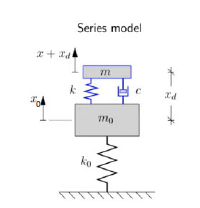
\includegraphics{image.png}

We will consider a footstep length of \(0.7 m\) {[}Bachmann et al.
(1997){]}, which means there will be, for a span of \(10 \text{ m}\),
\(n = \frac{10}{0.7} = 14.3\) cycles per span. For a damping ratio
\(\zeta = 0.02\), this represents a dynamic amplification factor of
\(\psi = 14.5\).

We also need to change the fourier coefficient \(\alpha\), which for a
person walking we will take \(\alpha = 0.4\)

\begin{Shaded}
\begin{Highlighting}[]
\NormalTok{psi }\OperatorTok{=} \FloatTok{14.5}
\NormalTok{alpha\_2}\OperatorTok{=}\FloatTok{0.4}

\CommentTok{\# Computing a\_max}
\NormalTok{a\_max\_2 }\OperatorTok{=}\NormalTok{ omega\_n}\OperatorTok{**}\DecValTok{2} \OperatorTok{*}\NormalTok{y}\OperatorTok{*}\FloatTok{1e{-}3} \OperatorTok{*}\NormalTok{ alpha\_2 }\OperatorTok{*}\NormalTok{ psi }\CommentTok{\#m/s²}
\NormalTok{display(Latex(}\SpecialStringTok{f"$a\_}\CharTok{\{\{}\SpecialStringTok{max, 2\}\} = }\SpecialCharTok{\{}\NormalTok{a\_max\_2}\SpecialCharTok{:.1f\}}\SpecialStringTok{ }\CharTok{\textbackslash{}\textbackslash{}}\SpecialStringTok{text}\CharTok{\{\{}\SpecialStringTok{ m/s²\}\}$"}\NormalTok{))}
\end{Highlighting}
\end{Shaded}

$a_{max, 2} = 1.8 \text{ m/s²}$

\textbf{Why is the response due to Load case 2 smaller than for Load
case 1 ?}

There are multiple reasons explaining why the response from load case 2
is smaller than the response from load case 1 :

\begin{itemize}
\tightlist
\item
  Firstly, a person walking generates less energy than a person jumping,
  which explains partly why the response is smaller.
\item
  Secondly, in load case 2 the person is considered to be walking
  accross the bridge. As such, the person is not always at the most
  efficient point (the middle of the bridge) and the number of cycles is
  limited. As such, the steady-state will not be reached.
\end{itemize}

\hypertarget{task-3--response-with-tuned-mass-damper-tmd}{%
\subsection{Task 3 : Response with Tuned Mass Damper
(TMD)}\label{task-3--response-with-tuned-mass-damper-tmd}}

The problem can be modelised as the following one (source: Week\#12 of
the lesson):

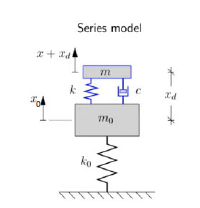
\includegraphics{image.png}

We are in the presence of a 2 degree of freedom system, with the first
degree of freedom corresponding to the SDOF calculed in Task 1 (on the
schema, with mass \(m_0 = m^*\), stifness \(k_0 = k^*\) and displacement
\(x_0 (t)\)) and the second degree of freedom being the TMD (with mass
\(m\), stiffness \(k\) and displacement \(x_d\)).

We are going to estimate the steady-state response of the bridge with
the TMD to an harmonic excitation with the natural frequency of the
bridge. As such, the excitation on the first degree of freedom will be
modelised as \(f(t) = f_0 \cdot e^{i\omega_n t}\).

As we are analysing the steady-state response, the response will have
the same frequency as the excitation, which yields :
\[ x_0(t) = x_0  \cdot e^{i\omega_n t} \rightarrow \ddot{x_0}(t) = - \omega_n^2 \cdot x_0 \cdot e^{i\omega_n t} \]

As such, the maximum acceleration will be
\(a_{max} = \omega_n^2 \cdot x_0\)

In order to get \(x_0\), we will compute the Dynamic Amplification
Factor, using the following result of the lesson : \[
DAF = \frac{\left|x_0\right|}{f_0 / k_0}=\frac{\sqrt{A^2+\left(2 \zeta_d\right)^2 B^2}}{\sqrt{C^2+\left(2 \zeta_d\right)^2 D^2}}
\]

With :

\begin{itemize}
\tightlist
\item
  \$A =
  \textbackslash omega\_0\^{}2\textbackslash left{[}\textbackslash omega\_d\^{}2-\textbackslash omega\^{}2\textbackslash right{]}
  \$
\item
  \(B = \omega_d \cdot \omega \cdot \omega_0^2\)
\item
  \(C = \omega^4-\left[\omega_0^2+(1+\mu) \omega_d^2\right] \omega^2+\omega_0^2 \omega_d^2\)
\item
  \(D = \zeta_d \cdot \omega_d \omega\left[\omega_0^2-(1+\mu) \omega^2\right]\)
\end{itemize}

And :

\begin{itemize}
\tightlist
\item
  \(\mu\) : Mass ratio (\(\mu=m / m_0\))
\item
  \(\zeta_d\) : Damping ratio of TMD
\item
  \(\omega_0\) : Frequency of structure (\(\omega_0 = \omega_n\))
\item
  \(\omega_d\) : Frequency of TMD
\item
  \(\omega\) : Frequency of excitation (\(\omega = \omega_n\))
\end{itemize}

As such, we can rewrite A, B, C, D :

\begin{itemize}
\tightlist
\item
  \$A = \textbackslash omega\_n\^{}2 \textbackslash omega\_d\^{}2 -
  \textbackslash omega\_n\^{}4 \$
\item
  \(B = \omega_d \omega_n^3\)
\item
  \(C = \omega_n^4-\left[\omega_n^2+(1+\mu) \omega_d^2\right] \omega_n^2+\omega_n^2 \omega_d^2 = - \mu \omega_d^2 \omega_n^2\)
\item
  \(D = \zeta_d \cdot \omega_d \omega_n \left[\omega_n^2-(1+\mu) \omega_n^2\right] = - \zeta_d \cdot \mu \cdot \omega_d \omega_n^3\)
\end{itemize}

\begin{Shaded}
\begin{Highlighting}[]
\CommentTok{\# Given}
\NormalTok{m\_d }\OperatorTok{=} \DecValTok{140} \CommentTok{\#kg}
\NormalTok{omega\_d }\OperatorTok{=} \FloatTok{2.44} \CommentTok{\#Hz}
\NormalTok{zeta\_d }\OperatorTok{=} \FloatTok{0.12}
\end{Highlighting}
\end{Shaded}

\begin{Shaded}
\begin{Highlighting}[]
\CommentTok{\# Compute A, B, C, D}
\NormalTok{mu }\OperatorTok{=}\NormalTok{ m\_d }\OperatorTok{/}\NormalTok{ m\_star}
\NormalTok{display(Latex(}\SpecialStringTok{f"$}\CharTok{\textbackslash{}\textbackslash{}}\SpecialStringTok{mu = }\SpecialCharTok{\{mu:.5f\}}\SpecialStringTok{$"}\NormalTok{))}

\NormalTok{A }\OperatorTok{=}\NormalTok{ omega\_n}\OperatorTok{**}\DecValTok{2} \OperatorTok{*}\NormalTok{ omega\_d}\OperatorTok{**}\DecValTok{2} \OperatorTok{{-}}\NormalTok{ omega\_n}\OperatorTok{**}\DecValTok{4}
\NormalTok{B }\OperatorTok{=}\NormalTok{ omega\_d }\OperatorTok{*}\NormalTok{ omega\_n}\OperatorTok{**}\DecValTok{3}
\NormalTok{C }\OperatorTok{=} \OperatorTok{{-}}\NormalTok{ mu }\OperatorTok{*}\NormalTok{ omega\_d}\OperatorTok{**}\DecValTok{2} \OperatorTok{*}\NormalTok{ omega\_n}\OperatorTok{**}\DecValTok{2}
\NormalTok{D }\OperatorTok{=} \OperatorTok{{-}}\NormalTok{ zeta\_d }\OperatorTok{*}\NormalTok{ mu }\OperatorTok{*}\NormalTok{ omega\_d }\OperatorTok{*}\NormalTok{ omega\_n}\OperatorTok{**}\DecValTok{3}

\BuiltInTok{print}\NormalTok{(}\StringTok{"A"}\NormalTok{, A, }\StringTok{"B"}\NormalTok{, B, }\StringTok{"C"}\NormalTok{, C, }\StringTok{"D"}\NormalTok{, D)}

\CommentTok{\#compute the DAF :}
\NormalTok{DAF }\OperatorTok{=}\NormalTok{ (A}\OperatorTok{**}\DecValTok{2} \OperatorTok{+}\NormalTok{ (}\DecValTok{2}\OperatorTok{*}\NormalTok{zeta\_d}\OperatorTok{*}\NormalTok{B)}\OperatorTok{**}\DecValTok{2}\NormalTok{)}\OperatorTok{**}\FloatTok{0.5} \OperatorTok{/}\NormalTok{ (C}\OperatorTok{**}\DecValTok{2} \OperatorTok{+}\NormalTok{ (}\DecValTok{2}\OperatorTok{*}\NormalTok{zeta\_d}\OperatorTok{*}\NormalTok{D)}\OperatorTok{**}\DecValTok{2}\NormalTok{)}\OperatorTok{**}\FloatTok{0.5}

\NormalTok{display(Markdown(}\SpecialStringTok{f"$DAF = }\CharTok{\textbackslash{}\textbackslash{}}\SpecialStringTok{frac}\CharTok{\{\{}\SpecialStringTok{|x\_0|\}\}}\CharTok{\{\{}\SpecialStringTok{f\_0/k\_0\}\} =  }\SpecialCharTok{\{}\NormalTok{right\_side}\SpecialCharTok{:.3f\}}\SpecialStringTok{$"}\NormalTok{))}
\end{Highlighting}
\end{Shaded}

$\mu = 0.06092$

\begin{verbatim}
A -84082.0611235632 B 12235.025278372217 C -106.25718064342774 D -89.4447229158234
\end{verbatim}

\begin{verbatim}
<IPython.core.display.Markdown object>
\end{verbatim}

We will consider, in a similar fashion to what we did in Task 2, that
the forcing function is the first harmonic of someone jumping, and
therefore that \$ f\_0 = \textbackslash alpha\_\{jumping\} *
\textbackslash mathrm\{G\} \$, with \(\mathrm{G} = 700 \text{ N}\)

With this result, we can compute \(\left | x_0 \right |\) and therefore
\(a_{max}\) :

\begin{Shaded}
\begin{Highlighting}[]
\NormalTok{f\_0 }\OperatorTok{=}\NormalTok{ alpha }\OperatorTok{*} \DecValTok{700} \CommentTok{\#N}

\end{Highlighting}
\end{Shaded}

\begin{verbatim}
1.7
\end{verbatim}
